\setchapterpreamble[or][.5\textwidth]{%
\dictum[ Donald E. Knuth]{%
Science is what we understand well enough to explain to a computer. Art is everything else we do.}\vskip1em}



\chapter{Fast GPU-based finite element solver}
%\epigraphhead[5]{\epigraph{ Science is what we understand well enough to explain to a computer. Art is everything else we do. }{Donald E. Knuth}}		

In this chapter, we present a set of novel methods to efficiently simulate corotated quadratic FE models in real-time. First, we address the problem how high resolution surface meshes can be mapped to quadratic isoparametric elements. In this scenario, the difficulty arises from the fact that the mapping from the reference element to each quadratic element is not bijective and not analytically invertible. Furthermore, there are far less elements in a higher order FE mesh than in a linear mesh if compared in terms of DOF. Therefore, it becomes more important to accurately extrapolate deformations to surface points outside the FE mesh. In this chapter, we present a novel mapping scheme to overcome this problem.

Massively parallel hardware (so called general purpose graphics processing units - GPGPU) have become a popular choice in recent years for speeding up time-critical algorithms in the realm of image processing and simulation. Although this hardware type offers a significantly higher performance in terms of floating point operations per second than traditional CPU architectures, the algorithms have to be carefully designed in order to fully exploit these resources. In particular, the algorithm has to be heavily parallelizable. In the following, an efficient GPU based solver for quadratic corotated tetrahedra is presented. For this purpose, we first introduce a matrix-free scheme in order to facilitate the implementation of a GPU based conjugate gradient (CG) solver. Then, we show how the performance of this solver can be greatly enhanced by using a parallel preconditioner based on the factorized sparse approximate inverse (FSAI). Finally, we present a novel GPU-based multigrid scheme to efficiently solve elasticity models on higher order, unstructured, non-conforming grids.

\section{Accurate surface embedding for higher order finite elements}
\label{AccurateSurfaceEmbeddingSection}

In this section a novel approach to accurately map highly detailed surface meshes to a higher order FE computational mesh is presented. The novel mapping scheme relies on a representation of each surface vertex in terms of a point on the computational mesh and its distance to the FE mesh in normal direction. Through this representation, the surface deformations remain smooth and local shape features are preserved even if very low-resolution FE meshes are used for computation. An efficient algorithm based on non-linear optimization is proposed to construct the mapping. We show that the algorithm performs robustly and that its numerical complexity is linear in the number of surface nodes and constant in the number nodes in the computational mesh.

The following description and evaluation of the novel mapping scheme is based on the corresponding proceedings publication \cite{Suwelack2013}.


\subsection{Closest point search in higher order meshes}

In order to facilitate the computation of the mapping later on, we first detail an efficient scheme to compute the closest point $\mbp (r,s,t)$ in the FE mesh $\mMesh$ for each vertex $\mVert$ of the triangular surface mesh $\mSMesh$. We will first show how to find $\mbp(r,s,t)$ for a single given vertex $\mVert$. Based on this results, a recursive mapping scheme will be introduced that can be used to compute $\mbp(r,s,t)$ for all $\mVert$ in $\mSMesh$.


The distance $d(r,s,t)$ from a point $\mbp(r,s,t)$ in the element $\mElem$ to an arbitrary surface vertex $\mVert$ is given by
\begin{equation}
d(r,s,t) = \left\| \mVert - \mathbf{x}_I N_I(r,s,t) \right\|.
\label{DistanceComputation}
\end{equation}


As $\mVert$ can be outside of $\mElem$, we have to constrict $(r,s,t)$ such that $\mbp(r,s,t)$ is indeed in $\mElem$. We can thus formulate the closest point search in terms of the constrained optimization problem 
\begin{align}
	&\min d(\mbp(r,s,t)) \quad \textnormal{s.t.} \nonumber \\
	&r>0, s>0, t>0 \quad \textnormal{and} \quad r+s+t \leq 1.
	\label{ConstrainedProblem}
\end{align}

As previously mentioned, the solution to this problem can be analytically determined if linear shape functions are used. For higher order shape functions, non-linear programming techniques have to be employed. We solve the constrained optimization problem (eq. X\ref{ConstrainedProblem}) using an extended Levenberg-Marquardt algorithm \cite{Nocedal1999} \cite{Kanzow2005}. The Jacobian is calculated using finite differences. It is important to point out that simple Newton-Raphson iterations are not guaranteed to converge even in the unconstrained case when $\mVert$ is inside $\mElem$.

The solution to problem (\ref{ConstrainedProblem}) can be described as the local optimum for $\mbp (r,s,t) \in \mElem$. The next step is to find the element $\mElem_{\min}$ where $\mbp (r,s,t)$ reaches its global minimum distance $d_{\min}$ in $\mMesh$. This can be efficiently accomplished with a recursive algorithm (see algorithm \ref{PointRecursionAlgo}).


\begin{algorithm}  
\caption{Recursively find $\mbp(r,s,t) \in \mMesh$}
\label{PointRecursionAlgo}
  \begin{algorithmic}
  % \Require Starting Element $\mathbb{E}_0$
	\Procedure{ClosestPoint}{$\mVert, \mElem, d_{\min}, \mElem_{\min}, \mathcal{T}$ }
	\State Solve (\ref{ConstrainedProblem}) to find closest point $\mbp$ with distance $d$
	\State to $\mVert$ in $\mElem$
	\If{$d < d_{\min}$}		
	\State $d_{\min} = d$, $\mElem_{\min} = \mElem$		
	\EndIf
	
	\If{$\mbp$ is on face of $\mElem$}
		\If{$\mbp$ is on surface of $\mMesh$}
			\If{$\mbp$ is on surface edge}
				\State Find neighbour tetrahedron $\mElem_1$ that contains
				\State surface triangle which shares edge				
				\EndIf
		\Else			
			\State Find tetrahedron $\mElem_1$ that shares face

		\EndIf
	
	
				\If{$\mElem_1$ exists and $\mElem_1 \notin \mathcal{T}$}				
				\State Add $\mElem_1$ to $\mathcal{T}$
				\State \Call{ ($\hat \mbp, \hat d, \hat{\mElem}$) = ClosestPoint}{$\mVert, \mElem_1, d_{\min}, \mElem_{\min}, \mathcal{T}$} 	
					\If{$\hat d < d_{\min}$}		
				\State $d =  \hat d$, $\mElem = \hat{\mElem}$, ${\mbp} = { \hat \mbp}$				
				\State $d_{\min} = d$, $\mElem_{\min} = \mElem$		
				\EndIf
			\EndIf
			
			\EndIf
	
			\Return $\mbp,d, \mElem$
			\EndProcedure
		
  \end{algorithmic}
\end{algorithm}

We first select an element $\mElem$ to start the iteration. Subsequently the closest point $\mbp \in \mElem$ to $\mVert$ is computed. This procedure is recursively called on the neighboring tetrahedra, if $\mbp$ is on a face of $\mElem$. The recursion is aborted if $d=0$ (i.e. $\mbp$ is inside the current tetrahedron) or if the neighbor tetrahedron that shares the face has already been visited (i.e. is in set $\mathcal{T}$). During each recursion step, the minimum distance $d_{\min}$ in $\mElem_{\min}$ is updated if a closer point $\hat \mbp$ is found.

The algorithm efficiently computes the local minimum distance $d_{\min}$ for a given initial guess $\mElem$. This local minimum coincides with the global minimum if the initial guess $\mElem$ is close enough to the real solution.




\subsection{Recursive mapping scheme}			

We now seek to not only map the whole surface mesh $\mSMesh$ to the computation grid, but also to reliable find the global minimum $d_{\min}$ for all $\mElem_i \in \mMesh$. For this purpose we introduce an outer recursion to the presented algorithm \ref{PointRecursionAlgo}. An initial mapping correspondence is established by finding the closest surface vertex $\mVert_0$ in $\mSMesh$ for an arbitrary point $\mbp_0$ in $\mElem_0$. It is important to point out that this inverse mapping problem is much easier to solve as the resolution of $\mSMesh$ is much higher than the resolution of $\mMesh$.

In order to start the outer recursion, we arbitrarily select an initial triangle $\mTri_0$ that contains $\mVert_0$. We than start a recursive scheme which maps all points in a given triangle $\mTri$ and uses the current mapping results ($\mbp, \mElem$) as the initial guess for mapping the neighbor triangles of $\mTri$ (see algorithm \ref{TriangleRecursionAlgo}).


\begin{algorithm}  
\caption{Recursively map triangles in $\mSMesh$}
\label{TriangleRecursionAlgo}
  \begin{algorithmic}
  % \Require Starting Element $\mElem_0$
	\Procedure{MapTriangle}{$\mTri, \mElem, d_{t}, \mathcal{P}$ }
	\State triangleMapped = true
	\ForAll{Surface vertices $\mVert$ in $\mTri$} 
	\If{$\mVert \notin \mathcal{P}$}
	\State Initialize empty $\mathcal{T}$, $d_{\min} = \inf$
	\State \Call{ ($ p,  d, \hat{\mElem}$) = ClosestPoint}{$\mVert, \mElem, d_{\min}, \mElem_{\min}, \mathcal{T}$} 		
	\If{$d<d_t$}
		\State $\mElem = \hat{\mElem}$ 
		\State Map vertex $\mVert$ to point $p$ in $\mElem$
		\State Add $\mVert$ to $\mathcal{P}$		
	\Else
		\State triangleMapped = false
	\EndIf	
	\EndIf
	\EndFor
	\If{triangleMapped}
	\ForAll{Neigbour triangles $\mTri_n$}
	\State \Call{ MapTriangle}{$\mTri_i, \mElem, d_{t}, \mathcal{P}$}
	\EndFor	
	\EndIf
	\Return
	\EndProcedure
		
  \end{algorithmic}
\end{algorithm}

The initial guess for each triangle depends on the mapping order of the triangles. Thus, there might be mapping orders that don't generate initial guesses which guarantee a global optimum for $d_{\min}$. That's why the mapping order is controlled by introducing the distance threshold $d_{t}$. The triangle $\mTri$ is only mapped (and the recursion only continues) if the distance for each surface vertex in $\mTri$ is below $d_{t}$. In order to make sure that all triangles are mapped, this distance threshold is incrementally raised until all triangles are mapped. 

For implementation purposes, the recursive scheme has to be unrolled into a loop in order to ensure an efficient and stable computation for large meshes.

\subsection{Accurate surface embedding}


We now define a scheme that maps the surface mesh $\mSMesh$ onto the computational mesh $\mMesh$ such that the deformed surface $\mSMesh'$ can be extrapolated from the deformed FE mesh $\mMesh'$ in a fast and correct way. For this purpose we represent each surface model vertex $\mVert$ in terms of a point $\mbp$ on the FE grid and its distance $d$ in normal direction (see Fig. \ref{MethodIllustration}). The deformed vertex position  
\begin{equation}
\mVert ' = \mbp ' + d \mbn '
\end{equation}
can subsequently be constructed using the position of $\mbp$ in the deformed configuration ($\mbp '$) as well as the deformed normal $\mbn '$. It will become apparent from the numerical examples that the proposed mapping preserves the smoothness of the deformation (and thus local shape features) even for surface regions that lie outside of the computational mesh.

\begin{figure}
   \centering   
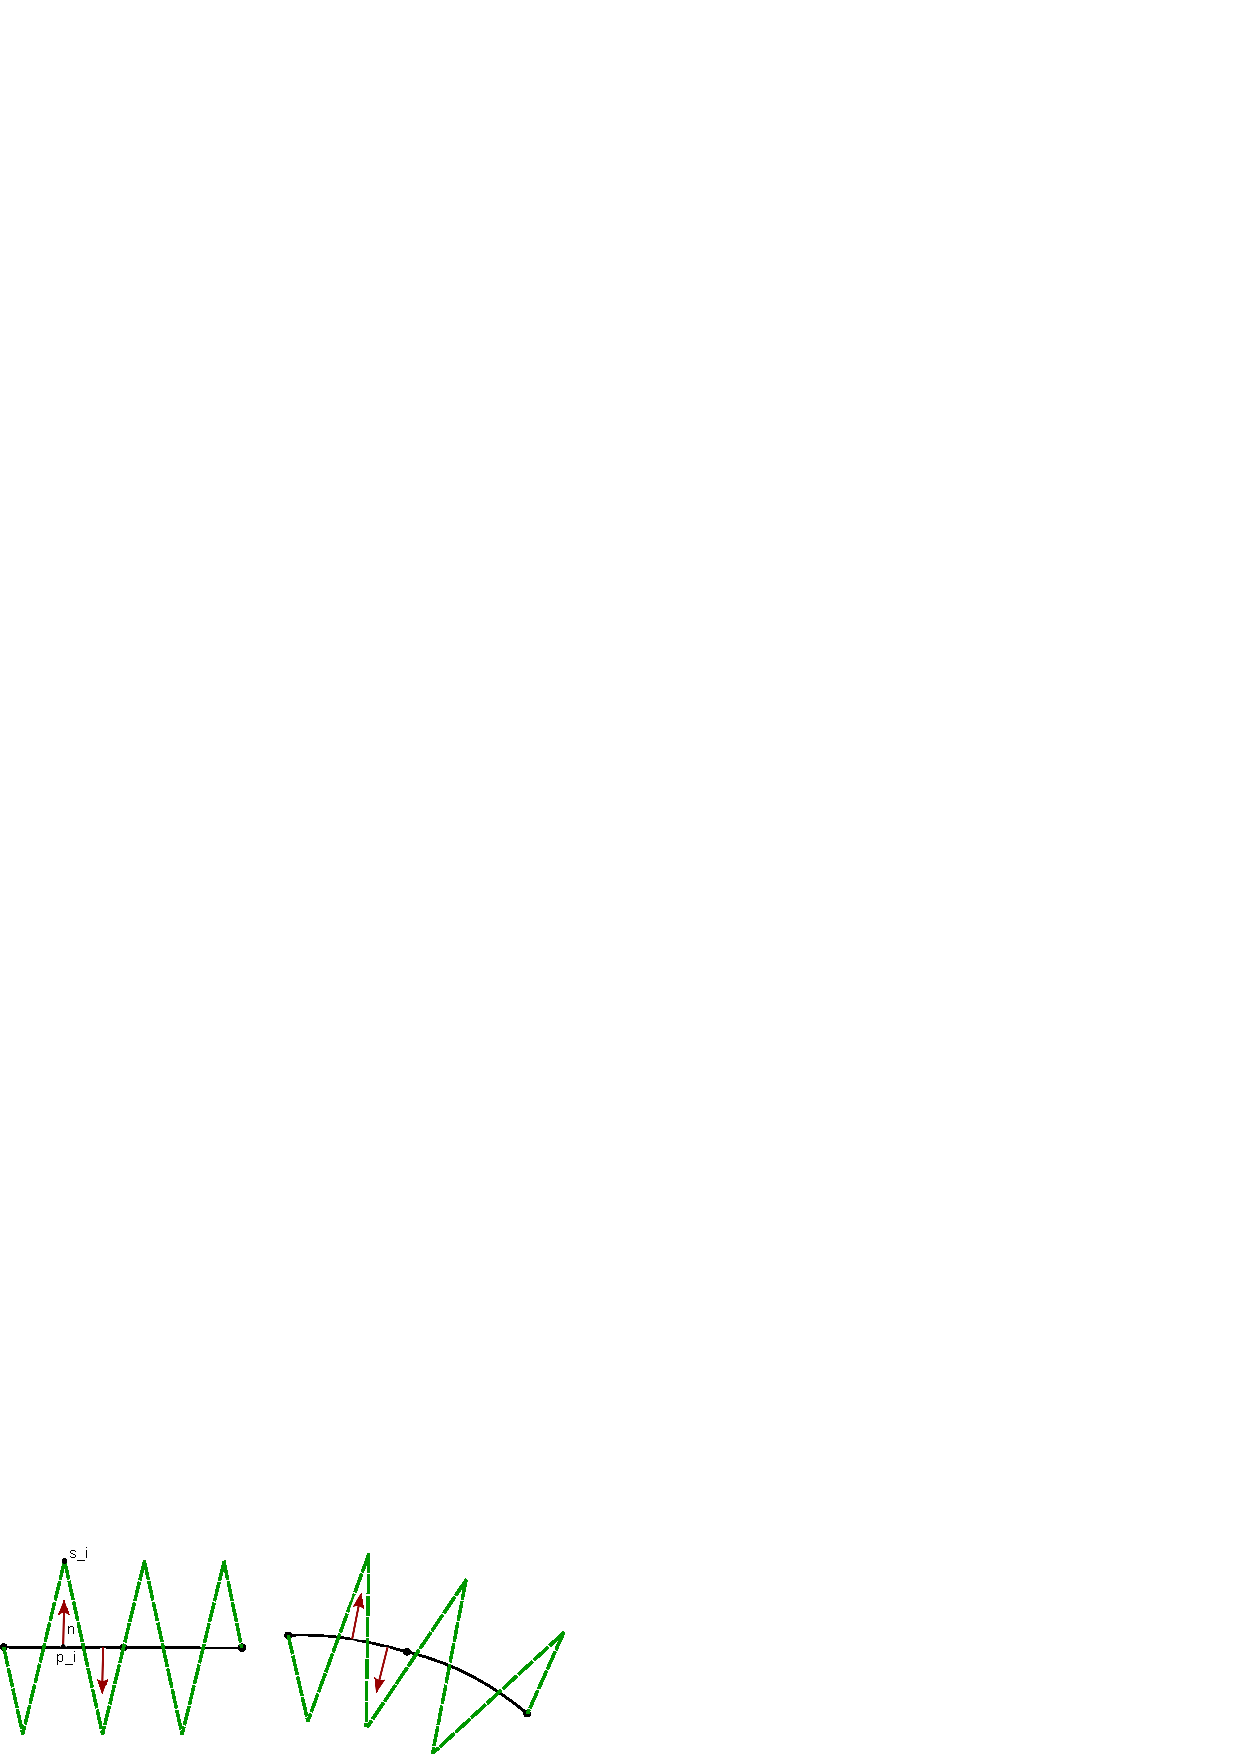
\includegraphics[width=\textwidth]{Figures/Seasaw.pdf}
\caption{Sawtooth surface attached to 1D quadratic edge. The deformation of the edge can be extrapolated to the surface while preserving local shape features.}
\label{MethodIllustration}
\end{figure}

\subsection{Smooth normal field}

At any surface point $\mbp$ on the mesh given in local coordinates $r, s$ with respect to the quadratic surface triangle, the spatial derivatives 
\begin{equation}
\frac{\partial \mbx (\mbp)}{\partial r} = \mathbf x_I \frac{\partial N_I (r,s)}{\partial r} \quad , \quad \frac{\partial \mathbf x (\mbp)}{\partial s} = \mathbf x_I \frac{\partial N_I (r,s)}{\partial s}
\end{equation}
can be calculated using the position of the nodes and the shape function derivatives at $r, s$ of the 6 node quadratic triangle. The normal $\mbn$ at $\mbp$ is then given by
\begin{equation}
\mbn  = \left( \frac{\partial \mathbf x (\mbp)}{\partial r} \times \frac{\partial \mathbf x (\mbp)}{\partial s} \right)/  \left\| \frac{\partial \mathbf x (\mbp)}{\partial r} \times \frac{\partial \mathbf x (\mbp)}{\partial s}  \right\|.
\label{NormalComputation}
\end{equation}

A smooth normal field is a necessary condition for the smoothness of the proposed mapping scheme. As the FE mesh is only $C^0$-continuous, the partial derivatives (and thus the normals) are discontinuous at element boundaries. Therefore, we average the normal at each node using the angle weighted average scheme. This results in an averaged normal $\overline{\mbn}_I$ for each surface vertex of the FE mesh and the normal 
\begin{equation}
\mathbf n  = ( \overline{\mbn}_I N_I(r, s) ) / \left\| \overline{\mbn}_I N_I(r, s) \right\|
\end{equation}
can be interpolated using the standard shape functions of the quadratic triangle. The smooth normal field that is created in this way can be efficiently computed. Furthermore, it is not necessary to re-compute the deformed vertex normals $\overline{\mbn}_I '$ every time step as shown in eq. (\ref{NormalComputation}). Instead, nodal rotation matrices can be defined at each node of the FE mesh which can be used to rotate the normal into the deformed configuration.


\subsection{Normal correction}

The aforementioned representation of each surface vertex $\mVert$ in terms of $(\mbp, d)$ can be obtained by solving a global optimization problem. The solution to this problem is not necessarily unique for complex, non-convex meshes. In order to construct the representation we first find the closest point $\mbp \in \mMesh$ to $\mVert$. Due to the normal smoothing, the normal $\mbn$ at $\mbp$ does not necessarily point in the direction of $\mVert$. Thus, we perform an additional correction step to make sure that the normal $\mbn$ at $\mbp$ does indeed point in the direction of $\mVert$. For this purpose we define the difference vector

\begin{equation}
\mathbold{\delta}(r,s,t) =  v_i - ( \mathbf{x}_I N_I(r,s,t) + d \cdot \mathbf{\overline{n}}_I N_I(r,s,t) ),
\label{NormalCorrectionComputation}
\end{equation}

where $d$ denotes the distance as defined in eq. (\ref{DistanceComputation}). The correction step can then be formulated in terms of the minimization problem 

\begin{align}
	&\min \mathbold{\delta}(r,s,t) \, \textnormal{s.t.} \nonumber \\
	&r>0, s>0, t>0 \, \textnormal{and} \, r+s+t \leq 1.
	\label{CorrectionProblem}
\end{align}

The optimization problem is solved in the same way as problem (\ref{ConstrainedProblem}): A recursive scheme along the lines of algorithm \ref{PointRecursionAlgo} is employed on top of a constrained Levenberg-Marquardt optimizer that uses finite differences to approximate the Jacobian.


\section{Matrix free conjugate gradient solver}

The necessary steps for solving the fully discretized scheme of the dynamic corotational formulation have already been outlined in section \ref{SectionProjectionBaedConstraints}. From this scheme, three computationally significant steps can be extracted: The computation of the nodal forces, the assembly of the stiffness matrix and the linear system solve. 


The nodal force computation consists of two stages. First, the elemental rotations are extracted and the elemental stiffness matrices are obtained through numerical integration. Afterwards, the elemental contributions are added to the nodal force vector. The whole process is inherently parallel and can be easily implemented on the GPU. In accordance with previous work (e.g. Allard et al. \cite{Allard2011}) we use one kernel launch to perform the elemental computations such as the polar decomposition of the deformation gradient and an additional kernel launch for the per-vertex gather operation. 


Implementing the matrix assembly and system solve step on the GPU is much more difficult. Most linear solvers (in particular the direct ones) do not parallelize well. For symmetric and positive definite systems an exception exists in the form of the conjugate gradient (CG) approach. This iterative method describes the linear system solve as a minimization problem for convex quadratic functions. The core ideas is to use so called conjugate directions instead of the local gradient for an efficient gradient descent minimization scheme \cite{Nocedal1999}. 


\begin{algorithm}  
\caption{Conjugate gradient algorithm for solving $\mathbf A \mathbf x = \mathbf b$}
\label{CGAlgo}
  \begin{algorithmic}
  % \Require Starting Element $\mathcal{E}_0$
	\State set $\mathbf x_0=0, \mathbf r_0 = \mathbf A \mathbf x_0- \mathbf b, \mathbf p_0 = -\mathbf r_0, k=0$ 
	\For{$k=0 < \textnormal{maxIter}$ } 
	\If{$\left\| \mathbf{r}_k \right\| / \left\| \mathbf{b} \right\| < \epsilon$}
		\State{break}
	\EndIf
	\State{$\alpha_k = \dfrac{\mathbf{r}^T_k \mathbf{r}_k}{\mathbf{Z}^T_k \mathbf{A} \mathbf{Z}_k} $ } 
	\State{$\mathbf x_{k+1} = \mathbf x_{k} + \alpha \mathbf p_{k}$} 
	\State{$\mathbf r_{k+1} = \mathbf x_{k} + \alpha \mathbf A \mathbf p_{k}$} 
	\State{$\beta_{k+1}=\dfrac{\mathbf{r}^T_{k+1} \mathbf{r}_{k+1}}{\mathbf{r}^T_k \mathbf{r}_k}$}
	\State{$\mathbf{Z}_{k+1} = -\mathbf{r}_{k+1}+\beta_{k+1} \mathbf{Z}_{k} $}
	\State{k=k+1}
	\EndFor
  \end{algorithmic}
\end{algorithm}


A basic sketch of the CG scheme (see Alg. \ref{CGAlgo}) reveals that only simple computational tasks such as vector addition, vector-vector multiplication and a (sparse) matrix-vector product are necessary for the system solve. In the context of an efficient GPU implementation, the most challenging part is the sparse matrix-vector product (SpMV) between the system matrix (see eq. \ref{LinearSystemNewmark}) and the current search direction $p_k$ in each CG step. In order to avoid a time-consuming matrix assembly, we don't build the system matrix every time step, but instead use a similar approach as Allard et al. \cite{Allard2011}: We first compute the per-element contributions for each nodal force and then accumulate these results for each node. In contrast to Allard et al. (and in contrast to the procedure for computing the nodal forces), we don't use a separate kernel launch for the per-vertex operations. Instead, we use a multi-coloring technique such that primarily those elements who do not share a common node are processed in parallel. With our layout it is still possible (although very rare) that the nodal force contributions of two elements of different color are updated simultaneously. We thus use an atomic operation in order to add these contributions to the nodal forces. As the atomic add causes virtually no overhead when no write conflicts occur, it is very efficient when used in combination with coloring techniques. 

The elemental contributions are computed by multiplying dense elemental matrices with corresponding nodal vectors. The performance of this kernel is limited by the memory bandwidth. In order to reduce the data transfer to global memory and to reduce the amount of shared memory used by each thread, we exploit the symmetry of the elemental matrices and use compressed matrices for data transfer. The matrix vector product is then performed using a constant lookup table for index mapping between the compressed and the uncompressed matrix.


\section{FSAI preconditioned conjugate gradients}
\label{PCGSection}

For inhomogeneous and stiff materials, the discrete elasticity problem becomes increasingly ill-conditioned, i.e. the condition number

\begin{equation}
\kappa (\mathbf{A}) = \left\| \mathbf{A} \right\|\cdot \left\| \mathbf{A}^{-1} \right\|
\end{equation}

becomes large. In this case, pure CG methods converge very poorly. A proven solution to this problem is to apply a preconditioner $\mathbf{Z}$\footnote{often denoted with $\mathbf P$ in the literature, we use $\mathbf Z$ to avoid confusion with the first Piola-Kirchhoff stress tensor} to the linear system. It is immediatly clear from  
\begin{equation}
\mathbf{Z}^{-1} \mathbf{A} \mathbf{dx} = \mathbf{Z}^{-1} \mathbf{b}
\end{equation}

that if $\mathbf{Z}^{-1}$ is close to $\mathbf{A}$, then $\mathbf{Z}^{-1}\mathbf{A}$ is near the identity matrix and the condition number $\kappa$ is low. If a preconditioner is used in a CG scheme, it has to be applied in each iteration, i.e. the equation

\begin{equation}
 \mathbf{Z} \mathbf{r} = \mathbf{z}
\label{PrecondApplication}
\end{equation}

has to be solved for the temporary vector $\mathbf{r}$ and the right hand side $\mathbf{z}$. That is why a key requirement for a good preconditioner is that its application according to eq. (\ref{PrecondApplication}) is fast and efficient. The Jacobi preconditioner therefore simply scales $\mathbf{A}$ with its inverse diagonal which means it uses the preconditioner $\mathbf{Z} = \textnormal{diag}(\mathbf{A})$.

A family of powerful preconditioners arises from the decomposition of $\mathbf{A}$ into triangular matrices. Every arbitrary square matrix can be written as the product of a lower and upper triangular matrix (LU decomposition). For symmetric, positive definite matrices the incomplete Cholesky (IC) decomposition 
\begin{equation}
\mathbf{A} \approx \mathbf{L}_A \mathbf{L}_A^T = \mathbf{Z}
\end{equation}

can drastically reduce the number of CG iterations for elastic problems \cite{Courtecuisse2010}. The application of the IC preconditioner requires two triangular solves of the sparse triangular matrices $\mathbf{L}_A,\mathbf{L}_A^T$. While this can be very efficient on the CPU, the triangular solve is inherently recursive, which makes a GPU implementation difficult.

The factorized sparse approximate inverse (FSAI) preconditioner is based on a different idea \cite{Kolotilina1993}. This method seeks to directly approximate the inverse of $\mathbf{A}$. In order to achieve this goal, $\mathbf{A^{-1}}$ is decomposed according to 

\begin{equation}
\mathbf{A^{-1}} \approx \mathbf{G}_L ^T \mathbf{G}_L = \mathbf{Z}^{-1}.
\end{equation}

In this context, the matrix $\mathbf{G}_L$ is an approximation the inverse of the lower Cholesky factor $\mathbf{L}_A$ in terms of the Frobenius norm $\left\| \mathbf{I}- \mathbf{G}_L \mathbf{L}_A  \right\|_F$. The approximation is constructed by minimizing the aforementioned Frobenius norm for a given sparsity pattern of $\mathbf{G}_L$. The commonly used FSAI(q) method uses the sparsity pattern of $\left| \mathbf{A} \right| ^q$.

The application of the FSAI preconditioner only needs two SpMV operations which are very fast on the GPU. It is clear that the more fill-ins are allowed in a higher order FSAI(q) scheme, the better is the approximation to $\mathbf{A^{-1}}$. However, at the same time the SpMV becomes increasingly time-consuming to compute. 

The biggest drawback of the FSAI preconditioner is its high set-up time. In the next section we describe how to overcome this problem.


\subsection{Preconditioner warping}
\label{PreconditionerWarping}
In the context of interactive simulations it is not feasible to compute the preconditioner every timestep, especially if complex schemes such as IC or FSAI are used. A better strategy is to compute the preconditioner just once and then appropriately adapt it every time step. For elasticity problems based on the corotated formulation, this can be efficiently achieved by local rotation warping of the preconditioner \cite{Courtecuisse2010}. The idea is based on the fact that the change in the system matrix $\mathbf{A}$ is dominated by the rotation warping of the elemental stiffness matrices (eq. \ref{CoRotStiffnessMatrix}). 

In order to apply these rotations to $\mathbf{Z}^{-1}$, we extract a local rotation $\mathbf{R}_n$ per node. We can subsequently define the global block diagonal rotation matrix $\mathbf{R}$ to formulate

\begin{equation}
\mathbf{R} \mathbf{Z}^{-1} \mathbf{R}^T \mathbf{A} \mathbf{dx} = \mathbf{R} \mathbf{Z}^{-1} \mathbf{R}^T \mathbf{b}.
\end{equation}

It is important to note that we do not have to explicitly compute $\mathbf{R} \mathbf{Z}^{-1} \mathbf{R}^T$ for each timestep, instead we serially apply the three operators. In this case it is not even necessary to build the global matrix $\mathbf{R}$, but each node can instead be rotated using the $3\times3$ matrix $\mathbf{R}_n$.

In the corotated FE model, the rotations are extracted on a per element basis. In order to compute the nodal rotations, we average the elemental rotations for each element around the node. This is done by first averaging the deformation gradient at the node before performing the rotation extraction according to Higham et al. \cite{Higham1988}. We have found this procedure to be more efficient than directly averaging the rotations using quaternions. In the case of quadratic tetrahedra, we use only the 4 corner vertices to compute the deformation gradient as explained in section \ref{QuadraticTetrahedraSection}.

Thanks to the warping scheme, the FSAI preconditioner can be computed in a pre-processing step from the linear stiffness matrix. It is even possible to store the preconditioner to disk and just load it at the beginning of each simulation.

The GPU implementation of the rotation warping and the subsequent application of the FSAI preconditioner is straight forward as the process is inherently parallel with a high data locality. As described above the rotation warping is performed by simply multiplying each node with a $3\times3$ rotation matrix. The application of the FSAI preconditioner requires two SpMV products. As the FSAI matrices do not change during the simulation, we just store them in GPU memory and apply them using a suitable CUDA library. 


\section{GPU-based multigrid solver for unstructured, non-conforming meshes}

The computational effort for the preconditioned conjugate gradient approach does scale superlinearly in terms of the number of mesh nodes (i.e. the DOF): Not only does the computational time for each PCG iteration increase, but the number of PCG steps increases as well for a fixed residual threshold. Thus, the method becomes inefficient for high resolution models. In contrast, multigrid methods can keep the computational effort proportional to the number of mesh nodes. The core idea is to efficiently remove low frequency errors by solving the linear system on a hierarchy of grids with different resolutions.

In this section, we present a novel multigrid scheme for efficiently solving elasticity problems using higher order FE on unstructured, non-conforming grids. We furthermore outline a set of methods that allows to efficiently implement the scheme on massively parallel architectures. In the following, we first give a brief general introduction to geometric multigrid schemes for solving linear systems that arise from elliptic PDEs. In this context we especially highlight the necessary components of the approach. Based on this discussion, we present a suitable prolongation/restriction scheme and a highly parallel smoothing scheme for simulations on unstructured grids. Finally, we detail a multigrid-preconditioned CG solver for the real-time simulation of deformable models.


\subsection{Basic multigrid scheme}

At the core of a multigrid solver lies a hierarchy of problem discretizations of different resolutions. This hierarchy consists of $l_{\textnormal{max}}$ levels with the associated system matrices $\mathbf A _l$. The solution scheme starts with an initial guess $\mbx _0$ on level $l=0$. In practice $\mbx _0$ is often chosen to be a vector of zeros or a value from a previous time step. The high frequency errors in this solution are subsequently attenuated by applying the smoothing operator $\mathcal{S}$. Typically, a variant of a fixed point iteration is used for this purpose (see section \ref{GPUBasedSmoothingSection} for details). In order to eliminate the low frequency errors, the remaining residual is consequently transferred to the next level $l+1$ with lower resolution. To do so, the residual $\mathbf r_l$ is first computed on the level $l$ and then transferred to the lower resolution mesh using the restriction operator $\mathcal{R}$ (refer to section \ref{MultigridHierarchySection} for more information). If the maximal mesh level $l_{\textnormal{max}}$ is reached, the remaining error $\mathbf e_{l+1}$ is determined by solving $\mathbf A _{l+1} \mathbf e_{l+1} = \mathbf r_{l+1}$ on the coarser mesh. This can be either done with a direct solver or using an iterative method such as the previously presented preconditioned gradient approach. If $l+1 < l_{\textnormal{max}}$, then the residual equation is recursively solved on the remaining levels of subsequently coarser meshes. In both cases, the error correction $\mathbf e_{l+1}$ is then transferred to the finer mesh at level $l$ by means of the prolongation operator $\mathcal{P}$. After adding the correction term $\mathbf e_{l}$ to the solution, a final smoothing step removes high-frequency errors that are introduced by the prolongation process.

In practice, several variants of the described multigrid scheme are used. First of all, the number of levels $l_{\textnormal{max}}$ can vary depending on the application. Furthermore, the described V-cycle is usually repeated several times until a given residual threshold is met. Finally, in many applications it is more efficient to spend more solving time on the coarse grids, thus leading to so called W-cycles. For a more detailed discussion on the basics of geometric multigrid methods we refer to appropriate textbooks \cite{Braess2007}.  

\begin{algorithm}  
\caption{V-cycle multigrid scheme for solving $\mathbf A \mathbf x = \mathbf b$}
\label{MGAlgo}
  \begin{algorithmic}
	\Procedure{MultigridSolve}{$\mathbf x_0 , \mathbf b , l$ }
	\State{${\mbx} \leftarrow \mathcal{S} (\mbx _0, \mathbf A_l, \mathbf b )$}	
	\State{$\mathbf r_l = \mathbf A _l {\mbx} - \mathbf b $}
	\State{$ \mathbf r _{l+1} \leftarrow \mathcal{R} (\mathbf r _l)$}
		\If{$l+1 < l_{\textnormal{max}}$}
		\State{InnerSolve $\mathbf A _{l+1} \mathbf e_{l+1} = \mathbf r_{l+1}$} 
	\Else
		\State { MultigridSolve({$\mathbf e _{l+1}, \mathbf b _{l+1}, l+1$ })}
	\EndIf	
	\State{$\mathbf e _l \leftarrow \mathcal{P} (\mathbf e _{l+1})$ }
	\State{$\mbx = {\mbx} + \mathbf e _l  $ }
	\State{${\mbx} \leftarrow \mathcal{S} (\mbx, \mathbf A_l, \mathbf b )$}	
	\State \Return{ \mbx }
	\EndProcedure	
  \end{algorithmic}
\end{algorithm}

\subsection{Multigrid hierarchy for non-conforming, higher order meshes}
\label{MultigridHierarchySection}

An accurate transfer of quantities between the meshes in the grid hierarchy is key in order to achieve an efficient multigrid scheme. For elasticity problems, the prolongation operator interpolates displacements between the meshes. The restriction operator transfers forces from a finer to a coarser grid. In many applications for geometric multigrid methods (especially in the realm of computational fluid mechanics), the finer mesh levels are constructed from an initial coarse mesh. In this way, all mesh levels cover the same region $\Omega_0$ (conforming mesh hierarchy). A construction of suitable prolongation and restriction operators is thus straight forward. Typically, these operators are linear and therefore have a matrix representation. In this context, the restriction operator is often chosen to be the transpose of the prolongation scheme. 

In order to accurately solve elasticity problems on unstructured grids, it is important to approximate the geometry as closely as possible. It is thus not desirable to construct the grid hierarchy from a coarse initial mesh. Instead, each mesh in the hierarchy should approximate the geometry as best as possible. Consequently, the meshes do not entirely overlap (non-conforming hierarchy) and thus displacements have to be extrapolated. When using linear tetrahedral grids, this can be achieved using barycentric coordinates \cite{Georgii2008}.

As outlined in section \ref{AccurateSurfaceEmbeddingSection} the interpolation and extrapolation of displacement and force fields that are defined on higher order isoparametric grids is more challenging. In our multigrid scheme, we use the previously presented mapping scheme based on the surface normal in order to interpolate the displacement between meshes (prolongation). In order to restrict the residual force vector to a coarser mesh, we do not make use of the surface normal. Rather, we map each nodal force to the corresponding element $\mElem$ in the coarse mesh that contains the closest point $\mbp (r,s,t)$ to the node. This force is then distributed among the nodes of $\mElem$ according to the basis function values at $\mbp (r,s,t)$.


\subsection{GPU-based smoothing}
\label{GPUBasedSmoothingSection}
The smoothing operators that are commonly used in geometric multigrid solvers can be expressed as fixed point iteration schemes. The idea of this class of iterative methods is to use the non-singular matrix $\mathbf B$ in order to express the linear system $\mathbf A \mbx = \mathbf b$ through
\begin{equation}
\mathbf B \mbx  + (\mathbf A - \mathbf B) \mbx = \mathbf b.
\end{equation}
The definition of the iteration 
\begin{equation}
\mathbf B \mbx ^{k+1}  + (\mathbf A - \mathbf B) \mbx^{k} = \mathbf b
\end{equation}
yields the update equation
\begin{equation}
\mbx ^{k+1} = \mbx^{k} - \mathbf B ^{-1} (\mathbf A \mbx^{k} - \mathbf b).
\label{MultigridUpdate}
\end{equation}

By decomposing $\mathbf A = \mathbf A_D + \mathbf A_L+ \mathbf A_U$ into the diagonal matrix $\mathbf A_D$ as well as the lower triangular matrix $\mathbf A_L$ and the upper triangular matrix $\mathbf A_U$, we can define two important smoothing schemes: Choosing $\mathbf B = \mathbf A_D$ yields the Jacobi method, while the Gauss-Seidel iteration scheme arises if $\mathbf B = \mathbf A_D + \mathbf A_L$. In a similar fashion as preconditioning techniques (see section \ref{PCGSection}), smoothing operators tend to work well, if $\mathbf B ^{-1}$ is a good approximation of $\mathbf A ^{-1}$. Thus, another class of commonly used smoothers are given by triangular decompositions of $\mathbf A$ such as $\mathbf B = \mathbf L \mathbf U$ (incomplete LU factorization) or $\mathbf B = \mathbf L \mathbf L^T$(incomplete Cholesky factorization).

It is apparent that the most efficient smoothers (e.g. Gauss-Seidel, ILU) rely on iteration schemes that are inherently recursive and thus not suitable for GPU implementation. For structured grids it is possible to divide the mesh into sets of non-neighboring elements (\emph{mesh coloring}) in order to parallelize the Gauss-Seidel method. However, this approach is very inefficient on unstructured grids. 

In order to facilitate a more efficient smoothing scheme, we use the previously presented FSAI technique ($\mathbf B^{-1} = \mathbf{G}_L ^T \mathbf{G}_L$). We again choose to precompute this decomposition and use the rotation warping technique to update the smoothing matrix for each time step. This results in a highly parallel algorithm that can be efficiently implemented on the GPU. In order to compute the SpMV product in the update equation (\ref{MultigridUpdate}), we again use the presented matrix-free scheme in order to avoid an assembly of the global system matrix.

\subsection{Multigrid-preconditioned CG for real-time elasticity}

We found that in many low-resolution elasticity problems, the prolongation leads to larger high-frequency errors near Dirichlet boundaries. Consequently, many smoothing steps are necessary, if the multigrid scheme is directly used for solving the linear system. An attractive alternative is to use the multigrid scheme as a preconditioner in a PCG algorithm. In this case, the accuracy of the multigrid iterations can be intentionally reduced. Thus it is enough to perform one V-cycle and 1 or 2 smoothing iterations within each preconditioning step. In order to achieve an efficient GPU implementation, we use the previously presented FSAI-preconditioned CG solver to perform the inner solve. Here, a residual threshold as high as 0.1 can be used without significantly degrading the performance of the solver. 


\section{Performance evaluations}

\subsection{Accurate surface embedding}

The novel mapping scheme was integrated into the SOFA framework \cite{Faure2012}. The constrained Levenberg-Marquardt implementation from the Levmar library was used to solve the minimization problem (eq. \ref{ConstrainedProblem}) \cite{LourakisJul.2004}. All simulations are run on a single core of an Intel i7-930 and we use nearly incompressible material models (Poisson's ratio $\nu=0.49$) in all scenarios.


\subsubsection{Accuracy}

The novel mapping scheme allows to accurately map high resolution surfaces to very low resolution quadratic tetrahedral grids. Fig. \ref{BunnySimulation} shows the deformation of the Stanford Bunny under gravity. It can be seen that the surface model mapped to a quadratic mesh with 1197 DOF deforms smoothly at the ears, although the computational mesh fails to approximate the geometry in this area. In contrast, the 9468 DOF tet4 model shows severe volume locking at the ears.

\begin{figure}
   \centering   
   \psfragfig[width=0.98\textwidth]{Figures/QuadraticTetrahedra/Bunny}
	\caption{Bunny surface mesh deforms under gravity. Volume locking is observed at ears for the simulation based on linear tetrahedra (left), while the tet10 mesh (middle) produces realistic and smooth surface deformations (right).}
\label{BunnySimulation}
\end{figure}

The gravity induced deformation of a seahorse model is considered as a second example. We construct different low resolution computational meshes from a high resolution surface mesh with 40k triangles: A linear tetrahedral (tet4) mesh with 258 DOF and 181 elements, a linear tetrahedral mesh with 992 elements and 1488 DOF as well as a mesh with 171 quadratic elements (tet10) and 1260 DOF (see Fig. \ref{SeahorseSimulation}). Barycentring coordinates are used in order to map the linear tetrahedral to mesh to the high resolution surface, while the presented mapping scheme is used to embed the tet10 mesh. As was apparent from the previous simulations of the beam geometry, linear meshes do not deform nearly as much as the quadratic FE mesh (volume locking effect). In order to ensure visually similar deformations, we thus subject the linear meshes to higher forces in order to overcome this artificial stiffness. 

\begin{figure}
   \centering   
   \psfragfig[width=0.98\textwidth]{Figures/QuadraticTetrahedra/SeahorseTet4AndTet10}
	\caption{Deformation of a seahorse model, from left to right: Linear tetrahedral FE mesh with 992 elements, the corresponding deformed surface mesh, a quadratic tetrahedral mesh with 171 elements and the deformed surface mesh mapped to the higher order FE mesh using the proposed mapping scheme.}
\label{SeahorseSimulation}
\end{figure}

For very low resolution tet4 meshes, the barycentric surface coupling results in large visible artefacts (see Fig. \ref{SeahorseSimulationCloseUp} left). In contrast, the proposed mapping scheme smoothly extrapolates the the deformation of the quadratic mesh is to the surface mesh and preserves local shape features. In case of the higher resolution tet4 mesh, the visible artefacts are substantially reduced. However, volumetric locking can still be observed at the end of the seahorse's tail. In contrast, the movement on the tail is much better captured by the quadratic mesh, also it has less DOF than the tet4 one (1260 vs. 1488). Furthermore, the barycentric mapping leads to a visible distortion of the seahorse's thorns even when using the higher resolution tet4 mesh (Fig. \ref{SeahorseSimulationCloseUp}). In contrast, the novel mapping scheme preserves the shape of the thorns. The dorsal fin of the seahorse is not included in the low resolution tet10 mesh and its deformation must thus be extrapolated during the simulation. Fig. \ref{SeahorseSimulationCloseUp} shows that this might lead to undesirable results even if the rotation invariant mapping is employed.


\begin{figure}
   \centering   
   \psfragfig[width=0.98\textwidth]{Figures/QuadraticTetrahedra/SeahorseCloseUp}
	\caption{Seahorse subjected to volumetric force: While the barycentric coupling leads to visible distortions (left, middle), the proposed mapping preserves local shape features (right).}
\label{SeahorseSimulationCloseUp}
\end{figure}


\subsubsection{Speed}

The performance and robustness of the approach is evaluated by mapping surface and volume meshes of different resolutions. We construct two volume meshes from the Asian dragon model that is included in the Stanford 3D scanning repository with 3000 elements and 1000 elements, respectively. Furthermore, surface models with mesh size from several thousands to several 100k elements are generated. The optimization algorithms robustly finds the correct surface representation (i.e. a point $\mbp$ on the computational mesh and the corresponding distance $d$) for all considered surface meshes. The convergence analysis (Fig. \ref{MappingConvergence}) confirms that the numerical complexity of the algorithm is linear in the number of surface nodes and independent of the size of the coarse computational mesh. 

Although the constrained Levenberg-Marquardt optimization that is run for each element is numerically complex, even large surface meshes with several 100k elements can be mapped in less than a minute thanks to the good convergence properties of the recursive scheme. Furthermore, the proposed surface representation can even be constructed in an offline process and the obtained coordinates can be simply loaded upon startup of the online simulation.

\begin{figure}
   \centering   
   \psfragfig[width=0.98\textwidth]{Figures/QuadraticTetrahedra/DragonConvergence}
	\caption{Different surface meshes are mapped to a 3000 element mesh (blue) and a 1000 element mesh (green). The mapping time is linear in the number of points of the surface mesh and independent of the computational mesh size.}
\label{MappingConvergence}
\end{figure}



\subsection{GPU based PCG solver}

The presented FSAI based GPU solver as well as Jacobi and ILU-preconditioned approaches were implemented using the SOFA framework \cite{Faure2012} and the Paralution library. All CPU computation are performed on a single core of an Intel i7-930, while the GPU implementation is run on a Tesla C2070. 

We again use the simple beam geometry under gravitational load (see Fig. \ref{BeamTwistAndGravity}) in order to assess the performance of the different solver configurations. We solve the dynamic problem with the Newmark integration method and scompute 200 time steps with a step size of $\Delta t = 0.05s$.

If the tet4 beam problem is solved using a CG-based scheme, the computation time of the nodal forces (right hand side) is negligible if compared to the linear system solve (see Fig. \ref{CGVsDirect}). For the 1461 DOF problem, the assembly of the nodal forces takes 10.39 ms on the CPU and the linear system solve is performed in 222.34 ms. Whereas for the smaller 1461 DOF problem only an acceleration factor of 1.3 is achieved by running the solver on the GPU, the large 58k DOF problem is solved more than 8 times faster on the GPU implementation. In case of the tet10 mesh, these observations are still valid, although the nodal force computations take about 10\% of the total solving time in this scenario. For this reason, the GPU speed-up is a bit higher for smaller problems (1.8x for the 2217 DOF beam). It can also be observed from Fig. \ref{CGVsDirect} that even the GPU-based Jacobi-preconditioned CG solver is heavily outperformed by the direct single-core Pardiso solver, which solves the 1461 DOF problem in 25 ms. 


\begin{figure}[htbp]
   \centering   
   \includegraphics[width=0.92\textwidth]{Figures/CGVsDirect.pdf}     
\caption{Solution times for the tet4 beam (top) and the tet10 beam (bottom). The complete solving time per time step for a Jacobi-preconditioned CG solver on the CPU (green) and on the GPU (red) is divided into the nodal force computations (dotted line) and the linear system solve (dashed line). Total solve time for the direct solver is shown in black.}
\label{CGVsDirect}
\end{figure}

As previously discussed, more complex preconditioners can speed up the CG scheme. Fig. \ref{PreconditionerComparison} shows that if an ILU preconditioner is used in conjunction with the presented rotation warping scheme, a speed-up by a factor of 3.6 can be obtained. Using the highly parallelizable FSAI approach leads to a speed-up of 1.7x in comparison to the Jacobi-preconditioned algorithm. For the purpose of real-time soft tissue registration it is not necessary to compute the exact solution of the linear system for each time step. By using a residual of 0.01 as the stopping criterion for the CG iterations, a sufficient accurate solution is obtained and the solution time can be significantly reduced (Fig. \ref{PreconditionerComparison} right). 

\begin{figure}[htbp]
   \centering   
   \includegraphics[width=0.92\textwidth]{Figures/PreconditionerComparison.pdf}     
\caption{Solution times for a CPU based CG solver scheme with a Jacobi (green), ILU (blue) and FSAI (red) preconditioner in comparison with a direct solver (black). The solution can be significantly speed up if a residual threshold of 1e-2 (bottom) is used for the CG scheme instead of computing the exact solution (top).}
\label{PreconditionerComparison}
\end{figure}



\begin{figure}[htbp]
   \centering   
   \includegraphics[width=0.92\textwidth]{Figures/PerformanceComparisonFinalGPUPardiso.pdf}     
\caption{Solution times for the tet4 beam (top) and the tet10 beam (bottom). Timings for the CPU based FSAI(2)-PCG solver (green) and the GPU variant of the algorithm (red) are listed as well as the total solve time for the direct Pardiso solver (black). }
\label{PerformanceComparisonFinalGPUPardiso}
\end{figure}

\subsection{GPU based multigrid solver}
We apply the proposed GPU based multigrid (MG) scheme to the beam model under gravitational load that was presented in the previous section. We analyze a discretization with 100120 tet4 elements (57915 DOF) and a tet10-based model with 8990 elements (41781 DOF). A residual of $0.01$ is used as the stopping criterion for the CG scheme. Furthermore, a grid hierarchy of 3 levels is used: For the tet4 beam the meshes consist of 100120, 8990 and 1810 elements, wheres the tet10 hierarchy is made up of meshes with 8990, 712 and 97 elements. For all MG computations, we use one iteration with a FSAI(2) scheme for smoothing purposes. The inner PCG solver uses an FSAI(2) preconditioner with rotation warping and a residual threshold of $0.01$.

The results of the computations are listed in Table \ref{TimingsMGComputations}. For comparison purposes, we also list the corresponding timings for the direct single-core Pardiso solver and the FSAI-preconditioned GPU-CG scheme that was extensively discussed in the previous section. As the nodal forces have to be computed on all levels in order to update the elemental stiffness matrices with the current rotation, their computation time ($t_{force}$) is slightly higher for the MG solver. However, the additional overhead stays well below $20\%$ for all scenarios. It is also apparent that the multigrid scheme is a very efficient preconditioner as the CG scheme only needs a few iterations to convergence. In contrast, the FSAI-PCG scheme needs an average of 115 (tet4) and 80 (tet10) iterations. In case of the CPU variant of the MG method, the largest amount of time is spent in the smoother (179 ms per time step for the tet4 model and 116 ms for the tet10 model). This component of the algorithm can be significantly accelerated by using GPU hardware (up to 9x for the tet4 model). In contrast, the acceleration of the inner PCG solve is not as pronounced. This is due to the low size of the inner problems, which do not utilize the full computational power of the GPU.

Overall it can be seen that the proposed GPU-based multigrid scheme is a very efficient solver. For the linear tetrahedral mesh, it achieves a speed-up of nearly 10x in comparison with the direct solver (5x in comparison with the CPU-PCG approach). For the quadratic tetrahedral discretization, this difference is even more pronounced: Here, a speed-up of more than 15x is obtained in comparison with the direct solver.


\begin{table*}
	\centering
		\begin{tabular}{cccccccccc}
				\hline & Solver &   $t_{force}$ & $t_{sm}$& $t_{in}$ & $t_{pre}$ & $t_{cg}$ & $n_{cg}$ & $t_{solve}$ & $t_{tot}$ \\\hline 
				 \parbox[t]{0.5mm}{\multirow{3}{*}{\rotatebox[origin=c]{90}{tet4}}}&Pardiso &  408&  & & & & & 2712& 3120 \\
				& GPU-PCG &  147& & & 5& 5 & 115 & 1314 & 1461\\
				&CPU-MG &  477 & 179 & 17&274&48&3&979&1476 \\
				&GPU-MG &  149 & 20 & 18 &54&5&3& 178&327 \\
				\hline
				 \parbox[t]{0.5mm}{\multirow{3}{*}{\rotatebox[origin=c]{90}{tet10}}}&Pardiso &  621& & & & & & 2001&2622 \\
				&GPU-PCG &  71& & & 5&2&80&574&645 \\
				&CPU-MG &  690&116&7&154&15&2&386&1076 \\
				&GPU-MG &  88&22&6&35&2&2 &84&172 \\
		\end{tabular}
	\caption{Computation times in ms for nodal force computation $t_{force}$, application time for preconditioner per CG step $t_{precond}$ (for MG solvers the computation times for the smoothing operator $t_{sm}$ and the inner solve $t_{in}$ are listed as well) and for one pure CG step $t_{cg}$. Additional columns list the number of CG steps $n_{cg}$, the total linear solver time $t_{solve}$ and the total computation time $t_{tot}$ per time step in ms.}
	\label{TimingsMGComputations}
\end{table*}

\section{Discussion}

In the previous chapter we have demonstrated that quadratic tetrahedral discretizations severely outperform linear tetrahedral meshes in terms of accuracy per number of degrees of freedom. Due to volume locking, the linear tetrahedral mesh needs more than a magnitude more (up to 40x) DOF in order to achieve the same accuracy as a tet10 mesh. In this chapter, a novel mapping scheme for embedding high resolution surface models into low-resolution higher order computational meshes was proposed. The mapping is constructed using a non-linear optimization algorithm whose complexity scales linearly with the number of vertices in the surface model and is nearly independent of the number of elements in the computational model.

The main contribution of this chapter is a fast GPU-based solver for quadratic corotated FE. Based on the novel mapping scheme for higher order isoparametric meshes, a novel multigrid approach for non-conforming, unstructured grids was presented. By using a novel FSAI-preconditioned CG solver as the coarse problem solver and employing a highly parallel smoothing scheme, the developed MG solver can be efficiently implemented on the GPU. The MG scheme significantly outperforms the direct Pardiso solver as well as the state-of-the-art Jacobi-preconditioned GPU-CG solver by more than an order of magnitude. It allows to simulate a high resolution, 8990 tet10 elements (41781 DOF) problem at nearly 6 time steps per second. As we will see in the upcoming chapter, this model size definitely provides sufficient accuracy in order to be used in a soft tissue registration scheme.
 


%
%\begin{table*}
	%\centering
		%\begin{tabular}{ccccccccccc}
				%\hline & Solver &  DOF &  $t_{force}$ & $t_{sm}$& $t_{in}$ & $t_{pre}$ & $t_{cg}$ & $n_{cg}$ & $t_{solve}$ & $t_{tot}$ \\\hline 
				 %\parbox[t]{2mm}{\multirow{3}{*}{\rotatebox[origin=c]{90}{tet4}}}&Pardiso & 57915 & 408&  & & & & & 2712& 3120 \\
				%& GPU-PCG & 57915 & 147.1& & & 4.79& 9.58 & 115.29 & 1836.57 & 1984\\
				%&CPU-MG & 57915 & 477.09 & 178.56 & 16.98 &274.33&47.56&3.04&978.55&1475.62 \\
				%&GPU-MG & 57915 & 148.5 & 20 & 18.26 &53.64&5.05&3.04& 178.42&326.92 \\
				%\hline
				 %\parbox[t]{2mm}{\multirow{3}{*}{\rotatebox[origin=c]{90}{tet10}}}&Pardiso & 41781 & 621.07& & & & & & 2000.98&2622.05 \\
				%&CPU-PCG & 41781 & 70.86& & & 5.23&4.71&79.87&819.47&890.33 \\
				%&CPU-MG & 41781 & 689.98&116.1&6.78&154.29&14.99&2.28&385.96&1075.94 \\
				%&GPU-MG & 41781 & 87.82&21.92&6.17&35.17&1.64&2.28 &83.93&171.75 \\
		%\end{tabular}
	%\caption{Computations times in ms for nodal force computation $t_{force}$, computation of nodal rotations $t_{nrot}$, application time for preconditioner per CG step $t_{precond}$ and for one pure CG step $t_{cg}$. Additional columns list the number of CG steps $n_{cg}$, the total linear solver time $t_{solve}$ and the total computation time $t_{tot}$ per time step in ms.}
	%\label{tab:Timings}
%\end{table*}




%Computation times for different algorithmic setups for the beam under gravity load are given in Table. \ref{tab:Timings}. All timings are averaged over 20 time steps. It can be seen that the number of CG  iterations $n_{cg}$ can be reduced by nearly an order of magnitude through the use of the FSAI preconditioner. The reduction is slightly more pronounced for the FSAI(3) preconditioned tet4 problems than for the FSAI(2) preconditioned tet10SR problems. However, the PCG approach requires the computation of the nodal rotations per time step ($t_{nrot}$) as well as the application of the preconditioner ($t_{precond}$) and its warping per CG step. While the additional nodal rotation warping is negligible and dominated by the kernel launch overhead (max. 0.08ms for all problems), the additional two SpMV multiplications needed for the preconditioner application substantially increase the computation time per CG step. Because of this increased computational complexity the speed-up related to the total linear solver time $t_{solve}$ for the PCG is about $5x$ for the tet4 problems and $3.5x$ for the tet10SR problems. It is important to point out that a residual of $1e-3$ was used as the stopping criterion for the CG iterations. A larger residual can be used in order to reduce the number of iterations for applications that don't require physical accuracy. However, there a minimal iteration count is required in order to maintain a stable simulation. It is also important to note that the reduction factor achieved through the use of a preconditioner remains approximately regardless of the enforced residual. For completeness, we list the time for the computation of the nodal forces $t_{force}$. These are dominated by the polar decomposition and the ensuing rotation of the element matrices. It is apparent that this step needs only little time in comparison with the linear system solve (especially for larger meshes). 
%
%\begin{table*}
	%\centering
		%\begin{tabular}{lcccccccccc}
				%\hline Model & Tetrahedra & DOF & Solver & $t_{force}$ & $t_{nrot}$  & $t_{precond}$ & $t_{cg}$ & $n_{cg}$ & $t_{solve}$ & $t_{tot}$ \\\hline 
				%Beam tet4 low & 4610 & 3222 & CPU CG & 16.91 & 0 &  0 & 2.33 & 798 & 1859 & 1876 \\
				%Beam tet4 low & 4610 & 3222 & CPU FSAI(3)-PCG & 16.44 & 2.6 &  1.72 & 2.39 &50 & 207.5  & 224 \\
				%Beam tet10SR low & 712 & 4002 & CPU CG & 61.15 & 0 &  0 & 2.16 & 1069 & 2309 & 2370 \\
				%Beam tet10SR low & 712 & 4002 & CPU FSAI(2)-PCG & 60.9 & 1.94 &  2.36 & 2.01 & 80 & 350 & 411 \\
				%Beam tet4 high & 19128 & 11982 & CPU CG & 69.58 & 0 &  0 & 11.21 & 1269 & 14225& 14295 \\
				%Beam tet4 high & 19128 & 11982 & CPU FSAI(3)-PCG & 69.57 & 12.23 &  8.25 & 10.65 & 147 & 2787 & 2865 \\
				%Beam tet10SR high & 4610 & 22002 & CPU CG & 378.3 & 0 &  0 & 12.99 & 1831 & 23785 & 24163 \\
				%Beam tet10SR high & 4610 & 22002 & CPU FSAI(2)-PCG & 378.8 & 11.7 &  16.52 & 12.56 & 242 & 7059 & 7436 \\
				%\hline
				%Beam tet4 low & 4610 & 3222 & GPU FSAI(3)-PCG & 4.72  & 3.38 & 0.31 &  0.67 & 50 & 49 & 53.72 \\
				%Beam tet10SR low & 712 & 4002 & GPU FSAI(2)-PCG & 16.54  & 2.25 & 2.84 &  0.82 & 80 & 90 & 107 \\
				%Beam tet4 high & 19128 & 11982 & GPU FSAI(3)-PCG & 20.7 & 4.5 &  1.03 & 1.51 & 147 & 373 & 394 \\
				%Beam tet10SR high & 4610 & 22002 & GPU FSAI(2)-PCG & 24.83 & 4.15 &  2.36 & 2.66 & 242 & 1215 & 1240 \\
		%\end{tabular}
	%\caption{Computations times in ms for nodal force computation $t_{force}$, computation of nodal rotations $t_{nrot}$, application time for preconditioner per CG step $t_{precond}$ and for one pure CG step $t_{cg}$. Additional columns list the number of CG steps $n_{cg}$, the total linear solver time $t_{solve}$ and the total computation time $t_{tot}$ per time step in ms.}
	%\label{tab:Timings}
%\end{table*}
%
%Table \ref{tab:Timings} also shows that the GPU implementation of the PCG algorithm is approx. 6x (tet10SR) to 7x (tet4) faster than the CPU implementation. The slightly higher speed-up for linear elements can be attributed to the fact that some parallelization strategies (e.g. coloring) depend on the number of elements rather than the number of nodes. In this context, the quadratic mesh sizes of 712 and 4610 elements respectively might even be too small to use the GPU to full capacity. Although our GPU code for nodal force computation isn't fully optimized it is apparent that for larger problems (tet10SR, 22002 DOF problem), this part of the FE simulation can greatly benefit from a GPU implementation.

%
%\section{Discussion}
%
%We have presented a detailed numerical and graphical comparison between linear and quadratic corotated finite elements for deformable body simulation. It is apparent that linear elements often need more than order of magnitude more DOFs to achieve the same accuracy than quadratic elements. This is not only true for high-resolution meshes, but also for small model sizes. In order to leverage the power of higher order isoparametric elements, we proposed a novel mapping scheme for embedding highly detailed triangular surface meshes to the computational grid. This mapping preserves local shape features and causes only negligible overhead during the simulation. It is constructed
%by representing each surface vertex in terms of points on the computational mesh and its distance to the FE mesh in normal direction. We proposed a recursive mapping scheme based on non-linear optimization to robustly construct this representation for curved isoparametric higher order FE meshes. The numerical complexity of the mapping scheme is linear in the number of surface nodes and independent of the size of the coarse computational mesh. 
%
%The numerical results show that the solution time of the FE algorithm is dominated by the linear solver. In order to speed up this component we presented an efficient GPU-based PCG algorithm. This is achieved by using an explicit, pre-computed preconditioner that is adapted for each time step using nodal rotation warping. Using the GPU-based approach, the complete FE simulation runs between $20x$ (quadratic elements) and $36x$ (linear elements) faster than a CPU based pure CG scheme. As the computational time for quadratic meshes is comparable to linear meshes with the same number of DOF, it is apparent that a combination of quadratic elements with the GPU based solver can yield speed-ups of more than two order of magnitude compared to a co-rotational method with linear shape functions on the CPU. 
%
%The main drawback of the method is the setup time for the FSAI preconditioner. If a single core implementation is used, the building of the preconditioner can take hours for larger meshes. This disadvantage can be alleviated by building the preconditioner offline in a precomputation step and just loading it from disk at the beginning of each simulation. Furthermore, recent work in this area shows that GPU implementation of the building phase can drastically reduce the setup time \cite{Dehnavi2012}.
%
%We would like to point out that the mapping scheme is neither restricted to quadratic elements nor to tetrahedral elements. The approach can be used to map highly detailed surface mesh to shell or volume meshes of arbitrary order and element type. The mapping approach might thus be able to facilitate the use of higher order elements for real-time simulations.   
%
%It is well known that multigrid based techniques constitute very efficient solving scheme for elastic problems \cite{Zhu2010}. Since these schemes scale linearly with the mesh size, they are especially useful for high resolution meshes. However, the implementation of multigrid schemes on the GPU for unstructured grids is challenging. We would like to emphasize that the contributions of this paper provides the two essential blocks for a GPU-based multigrid scheme for unstructured higher order FE meshes. Not only can the proposed mapping technique be used to transfer displacements between the grids at different resolution, but the FSAI preconditioner can also be used as a smoother in a multigrid scheme \cite{Heuveline2012}. Thanks to the rotation warping technique, FSAI based smoothing can be used in real-time simulations.



  
